% Options for packages loaded elsewhere
\PassOptionsToPackage{unicode}{hyperref}
\PassOptionsToPackage{hyphens}{url}
%
\documentclass[
  oneside]{ubcthesis}
\usepackage{lmodern}
\usepackage{amssymb,amsmath}
\usepackage{ifxetex,ifluatex}
\ifnum 0\ifxetex 1\fi\ifluatex 1\fi=0 % if pdftex
  \usepackage[T1]{fontenc}
  \usepackage[utf8]{inputenc}
  \usepackage{textcomp} % provide euro and other symbols
\else % if luatex or xetex
  \usepackage{unicode-math}
  \defaultfontfeatures{Scale=MatchLowercase}
  \defaultfontfeatures[\rmfamily]{Ligatures=TeX,Scale=1}
\fi
% Use upquote if available, for straight quotes in verbatim environments
\IfFileExists{upquote.sty}{\usepackage{upquote}}{}
\IfFileExists{microtype.sty}{% use microtype if available
  \usepackage[]{microtype}
  \UseMicrotypeSet[protrusion]{basicmath} % disable protrusion for tt fonts
}{}
\makeatletter
\@ifundefined{KOMAClassName}{% if non-KOMA class
  \IfFileExists{parskip.sty}{%
    \usepackage{parskip}
  }{% else
    \setlength{\parindent}{0pt}
    \setlength{\parskip}{6pt plus 2pt minus 1pt}}
}{% if KOMA class
  \KOMAoptions{parskip=half}}
\makeatother
\usepackage{xcolor}
\IfFileExists{xurl.sty}{\usepackage{xurl}}{} % add URL line breaks if available
\IfFileExists{bookmark.sty}{\usepackage{bookmark}}{\usepackage{hyperref}}
\hypersetup{
  pdftitle={Trajectory planning with real time vision-based obstacle detection},
  pdfauthor={Xuemeng Li},
  hidelinks,
  pdfcreator={LaTeX via pandoc}}
\urlstyle{same} % disable monospaced font for URLs
\usepackage{longtable,booktabs}
% Correct order of tables after \paragraph or \subparagraph
\usepackage{etoolbox}
\makeatletter
\patchcmd\longtable{\par}{\if@noskipsec\mbox{}\fi\par}{}{}
\makeatother
% Allow footnotes in longtable head/foot
\IfFileExists{footnotehyper.sty}{\usepackage{footnotehyper}}{\usepackage{footnote}}
\makesavenoteenv{longtable}
\setlength{\emergencystretch}{3em} % prevent overfull lines
\providecommand{\tightlist}{%
  \setlength{\itemsep}{0pt}\setlength{\parskip}{0pt}}
\setcounter{secnumdepth}{5}
\previousdegree{B.A.Sc., Simon Fraser University, 2017}

\usepackage{booktabs}
\usepackage{makeidx}
\usepackage{graphicx}
\usepackage{makecell}



\makeindex
\frontmatter
\usepackage[]{natbib}
\bibliographystyle{apalike}

\title{Trajectory planning with real time vision-based obstacle detection}
\author{Xuemeng Li}
\date{April 2020}

\begin{document}
\maketitle


\noindent The following individuals certify that they have read,
and recommend to the Faculty of Graduate and Postdoctoral Studies
for acceptance, the thesis entitled:

\begin{center}
{\large \textbf{Trajectory planning with real time vision-based obstacle detection}}
\end{center}

submitted by \textbf{Xuemeng Li} in partial fulfillment of the requirements for the degree of \textbf{Master of Engineering} in \textbf{Electrical and Computer Engineering}.%
\par\bigskip%

\noindent\textbf{Examining Committee:}%
\par\medskip\noindent{Maryam Kamgarpour, Electrical and Computer Engineering, UBC}\\\emph{Supervisor}
\par\medskip\noindent{Mahdi Yousefi, Avestec Technologies Inc.}\\\emph{Supervisor}
\cleardoublepage

\chapter{Abstract}

Autonomous aerial vehicles are broadly used to assist human in dangerous or complex monitoring tasks, such as inspection of hard to reach high voltage power lines and oil pipes, monitoring and distinguishing wildfire, or improving precision farming. An autonomous navigation system can support drones or robots to move towards targeted positions without any external control. A fully functional autonomous system requires an integration on a wide range of algorithms, including trajectory planning algorithms, object detection with image processing and robust control algorithms for path following. 

In this project, an implementation of trajectory planning with object detected from the video with depth information has been described. The location and size of the targets are determined through image processing and convex optimization with the depth information collected from Intel Real Sense Camera. Then the trajectory planning function based on Rapid-exploring random tree (RRT) algorithm will plan the path on the map which combined the detected obstacle according to the obstacle detection function. This process would ensure drones or robots reaching the target domain safely.

{
\setcounter{tocdepth}{2}
\tableofcontents
}
\hypertarget{list-of-abbreviations}{%
\chapter{List of Abbreviations}\label{list-of-abbreviations}}

\begin{longtable}{ll}
\toprule
Short & Long\\
\midrule
RRT & Rapid-exploring Random Tree\\
RGB & Red green blue additive color model\\
ROS & Robot Operating System\\
SDK & Software development kit\\
FOV & Field of View\\
\bottomrule
\end{longtable}

\hypertarget{acknowledgements}{%
\chapter{Acknowledgements}\label{acknowledgements}}

I would like to thank the supervision of Dr.~Maryam Kamgarpour and Dr.~Mahdi Yousefi.

\mainmatter

\hypertarget{introduction}{%
\chapter{Introduction}\label{introduction}}

Autonomous aerial vehicles and robotics are broadly used to provide human assistance on dangerous or complex tasks. Fields such as oil, mining, wildfire extinguishing, and precision farming are requiring more robotic involvement nowadays. To better adapting to duties' requirements, an autonomous navigation system is essential for the robots or drones to safely accomplish the work with minimal human control. In this project, an integration of the obstacle detection and trajectory plan has been implemented as the start point for the autonomous navigation system for future integration on robot's hardware.
One of the main algorithms used in this project is the Rapid-exploring random tree (RRT) algorithm for path planning. Initially brought up by Steven M. LaVell and James J. Kuffner Jr {[}5{]}, the RRT algorithm could efficiently search nonconvex and high-dimensional spaces by constructing space-filling tree from samples drawn randomly in the search space and inherent grows towards large unsearched areas. The algorithm has been broadly discussed and implemented in education materials for robotics such as Python Robotics {[}1,2{]}. Many variants and improvements for motion planning have been studied and implemented. There are also comparison researches on improving the RRT algorithms {[}6{]}. With all these variants, the original RRT algorithm holds its tidy and simplicity which is good to be used as a start point. Therefore, in this project, original RRT algorithm has been implemented as object-oriented with MATLAB. In original RRT algorithm, the next point of the tree is generated based on the direction to random point, selected step size and whether is on the obstacle.

The intel RealSense Camera D400 series is a stereo vision depth camera system {[}7{]}. The small size and ease of integration of the camera sub system provides integration flexibility on wide range of products including drones, robots, virtual reality, PC peripherals and home surveillance. Works have been done for image processing with RealSense Camera. For example, Chang utilized the OpenCV DNN object detection package within RealSense Camera to outline the obstacles in RGB content in real-time {[}3{]}. To better utilize the depth information, Song and Xiao implemented depth maps for object detection and designed a 3D detector to overcome the difficulties for recognition based on rendering hundreds of viewpoints of a CAD model to obtain synthetic depth maps {[}4{]}. In this project, Intel's RealSense Depth Camera D435i has been used for object detection because of its handy size, ease of integration with cross-platform open source Intel RealSense SDK application and stereo depth camera which designed to maintain its calibration throughout lifetime.

In the following sections of this report, detailed implementation process and discussion on the results will be described. For algorithm implementation, there will be explanations on how to generate an RRT tree for trajectory plan, how to identify the obstacle with the depth video file from RealSense camera and how to integrate the image processing with the trajectory plan. The accuracy of the measurement for the camera will also be discussed. And in the section after, detailed assessment of the work including error source, advantages and disadvantages, and future steps for improvements will be discussed.
\citep{meyer2003pressures}.

\hypertarget{algorithm-and-implementation}{%
\chapter{Algorithm and Implementation}\label{algorithm-and-implementation}}

The implementation of the project has been done in MATLAB. Rapid-exploring Random Tree Algorithm has been implemented for trajectory plan and object detection algorithm has been built with depth information extracted from RealSense Camera. The overall implementation has been committed to GitHub at \textbf{\href{https://github.com/luckymeng7/EECE597}{this link}}

\hypertarget{rapid-exploring-random-tree-algorithm-for-pathway-planning}{%
\section{Rapid-exploring Random Tree Algorithm for Pathway Planning}\label{rapid-exploring-random-tree-algorithm-for-pathway-planning}}

Rapid-exploring Random Tree (RRT) algorithm was introduced by Steven M. LaVell and James J. Kuffner Jr {[}5{]}. To efficiently search nonconvex and high-dimensional spaces, the algorithm constructs a space-filling tree from samples drawn randomly in the search space and inherently grows towards large unsearched areas.

The output of the RRT algorithm is a tree(T) that contains all of the randomly sampled nodes(q) with connection to their inherit points. With object-oriented programming, each of the sampled node has been assigned as a class of Node with properties of index, parent index, position and path to node. An RRT class is defined to contain all generated nodes, with properties of total number of the nodes, initial node, positions of all existing node and a list of all existing nodes. A new node will be sampled in each iteration and the RRT tree will be updated if the path to this new node has avoided the obstacle. To generate a new node(qnew), a random point(qrand) will be firstly generated within the map range. Then it will be connected to the nearest node(qnear) on the tree. On the connection line, a point with max-step distance (step size) to the nearest point will be selected as the new node if it is confirmed as clear with obstacle free function. Figure \ref{fig:figure1} shows the generation of one new node to the tree.

\begin{figure}

{\centering 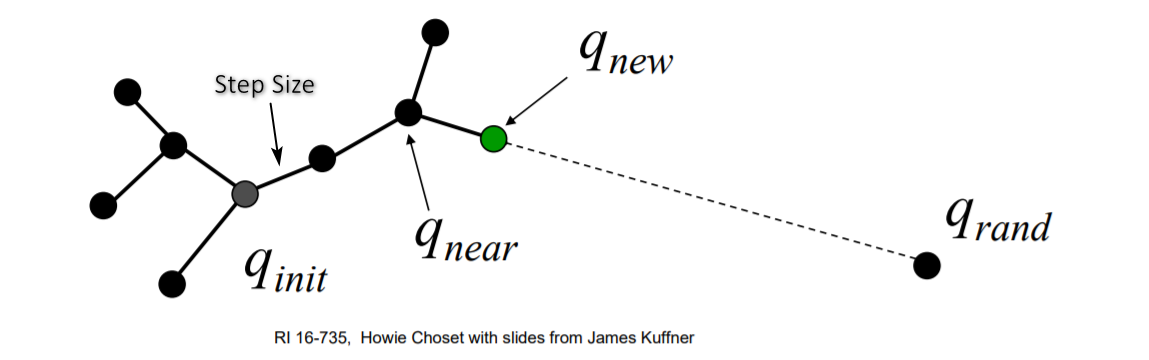
\includegraphics[width=0.6\linewidth]{figures/1} 

}

\caption{New Node Generation}\label{fig:figure1}
\end{figure}



For a general configuration space, the algorithm in pseudocode is as follow {[}6{]}:

\begin{verbatim}
Algorithm T=(V,E) ← RRT*(qini)
T ← InitializeTree();
T ← InsertNode(𝜱, qini, T);

    for i = 1 to K do
        qrand ← RAND_CONF()
        qnearest ← NEAREST_VERTEX(qrand, T)
        qnew ← STEER (qnear, qrand, Δq)
          if Obstaclefree(qnew) then
            qnear ← Near(∆D, qnew, T);
        qmin ← Chooseparent(qnear, qnew, qnearest);
        T ← InsertNode(qmin, qnew, T);
        T ← Rewire(T,qmin, qnew, qnear);
      
    return T
\end{verbatim}

\begin{itemize}
\tightlist
\item
  ``←'' denotes assignment. For instance, ``largest ← item'' means that the value of largest changes to the value of item.
\item
  ``return'' terminates the algorithm and outputs the following value.
\end{itemize}

The inputs for the algorithm are initial position, destination position, max step size, obstacle size and position and the overall map size. The output for the function is a planned path and the overall tree.

Real-time obstacle detection has also been implemented. As the robot moving forward, the function would recalculate the tree when it detects a new obstacle shows up. The current position would be taken as the new start point and the destination position would still be the same. Figure \ref{fig:figure2} shows path updated by twice after initial path planned.

\begin{figure}

{\centering 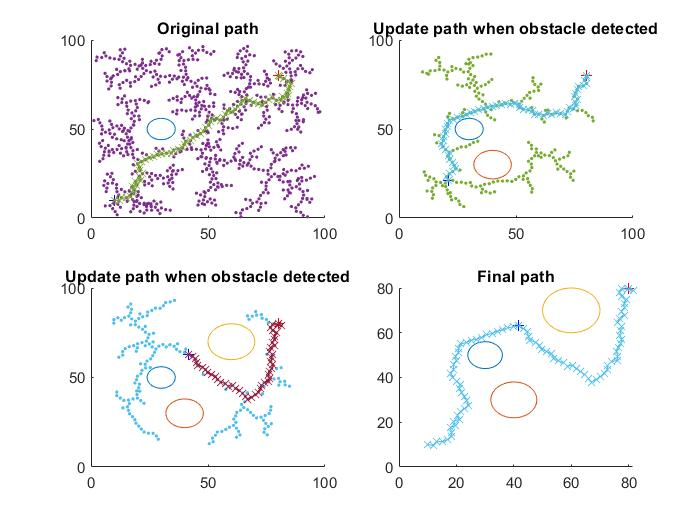
\includegraphics[width=0.7\linewidth]{figures/2} 

}

\caption{Path updated when new obstacle detected}\label{fig:figure2}
\end{figure}



\hypertarget{image-processing-for-obstacle-detection}{%
\section{Image Processing for Obstacle Detection}\label{image-processing-for-obstacle-detection}}

With the video stream captured with Intel RealSense camera, the depth information could be used for object detection. With MATLAB's ROS toolbox, the bag video was imported and processed as depth frames and RGB frames. A function has been implemented to identify the obstacle based on the depth information. On each of the frames, a mask will be created as any pixels that has depth value within the sensitive detection range will be set to 100 and the rest pixels will be set to 0. The comparison between regular RGB image and detected obstacle area are shown in figure \ref{fig:figure3}

\begin{figure}

{\centering 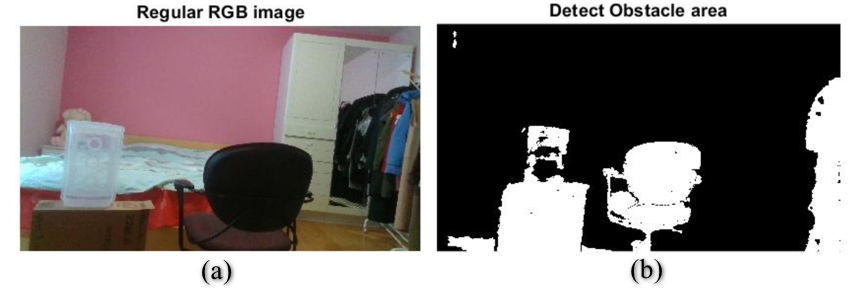
\includegraphics[width=0.8\linewidth]{figures/3} 

}

\caption{Obstacle detected in depth field}\label{fig:figure3}
\end{figure}



In order to project the obstacles properly onto the map where the trajectory is planned, top views for each frame are created. By looping through the columns number of the depth image, using the smallest depth value of each column as the row number and assign row number of the related point to the value of that pixel for the top view. A distance threshold is used to set the limitation of the depth size. For example, currently, only objects within two meters distance would be captured as object and saved in top view as figure \ref{fig:figure4}.

\begin{figure}

{\centering 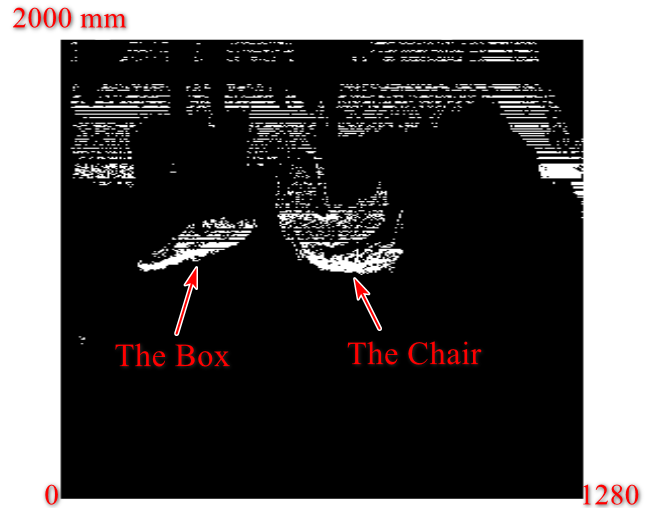
\includegraphics[width=0.3\linewidth]{figures/4} 

}

\caption{Top view based on depth information}\label{fig:figure4}
\end{figure}



Output videos are created by combining frames of top views or obstacle masks on the RGB frames.

\hypertarget{measurement-and-calculation-of-the-object-size}{%
\section{Measurement and Calculation of the Object Size}\label{measurement-and-calculation-of-the-object-size}}

Based on the datasheet of the RealSense camera {[}7{]}, the horizontal field of view (FOV) for depth image is 74 degree and vertical field of view for depth image is 62 degree. Based on the definition of FOV in figure \ref{fig:figure5} as follow:

\begin{figure}

{\centering 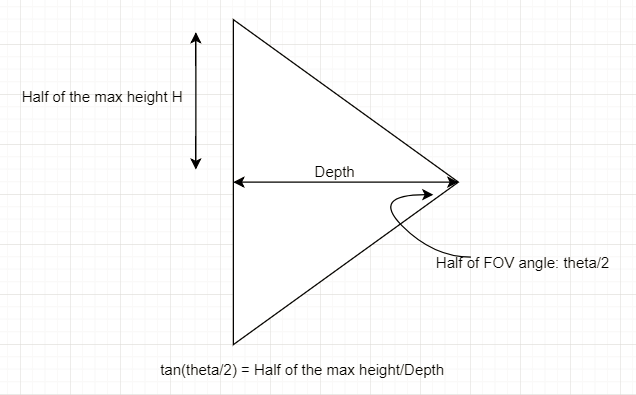
\includegraphics[width=0.6\linewidth]{figures/5} 

}

\caption{Definition of field of view}\label{fig:figure5}
\end{figure}



the actual width and height based on the pixel value could be calculated as:

\[ Actual width = \frac{width \space pixel}{resolution \space on \space width} \cdot depth \cdot \tan(\frac{74}{2}) \cdot 2 \]

\[ Actual height = \frac{height \space pixel}{resolution \space on \space width} \cdot depth \cdot \tan(\frac{74}{2}) \cdot 2 \]

In order to use actual size as base point to do the calibration, I transferred the above equations into:

\[ \tan(x) = \frac{rp \cdot L1}{l1 \cdot D1} \]

Where
- rp is the resolution on width or height direction,
- L1 is the actual width or height,
- l1 is the pixel number on width or height,
- D1 is the actual depth distance.

Another transfer for the equation would become:
\[\frac{L1}{l1 \cdot D1} = \frac{L2}{l2 \cdot D2} = C\]

The table \ref{tab:mytable1} are the measurements that I used to calibrate the measurement with resolution 1280x720 for both depth image and RGB image. The measurement of actual height and width are done with a ruler on the object and the measurement of height and width in pixel is measured on the image directly. The depth value of the center point on the has been used as the depth info for the overall object. The unit for actual measurements is millimetre:

\begin{table}

\caption{\label{tab:mytable1}Measurements for calibration}
\centering
\begin{tabular}[t]{lrrr}
\toprule
Item Number & 1.00e+00 & 2.00e+00 & 3.00000\\
Depth(mm) & 4.15e+02 & 2.97e+02 & 683.00000\\
Height(Actual) & 7.50e+01 & 9.00e+01 & 252.00000\\
Height(Pixel) & 1.71e+02 & 2.70e+02 & 336.00000\\
Ch & 1.06e-03 & 1.12e-03 & 0.00109\\
\addlinespace
Width(Actual) & 2.25e+02 & 1.42e+02 & 173.00000\\
Width(Pixel) & 4.89e+02 & 4.35e+02 & 227.50000\\
Cw & 1.11e-03 & 1.09e-03 & 0.00111\\
\bottomrule
\end{tabular}
\end{table}

Figure \ref{fig:figure6} are the images for the above objects (1,2,3 from left to right):

\begin{figure}

{\centering 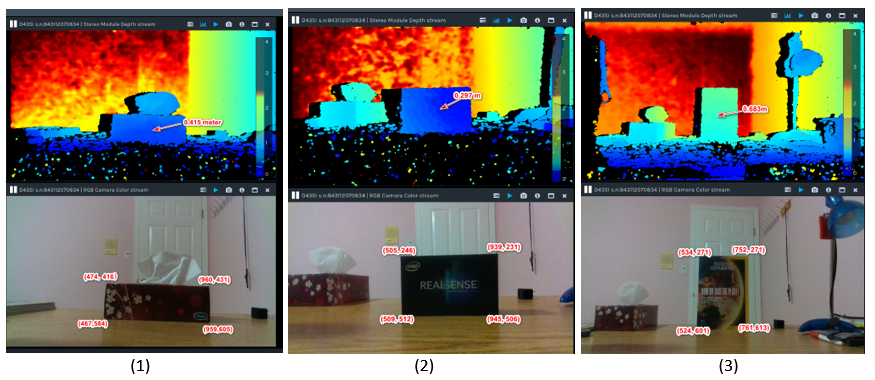
\includegraphics[width=0.9\linewidth]{figures/6} 

}

\caption{Definition of field of view}\label{fig:figure6}
\end{figure}



To calculation with equation \[\frac{L1}{l1 \cdot D1} = \frac{L2}{l2 \cdot D2} = C\], the following three objects in figure \ref{fig:figure7} are measured (4, 5, 6 from left to right):

\begin{figure}

{\centering 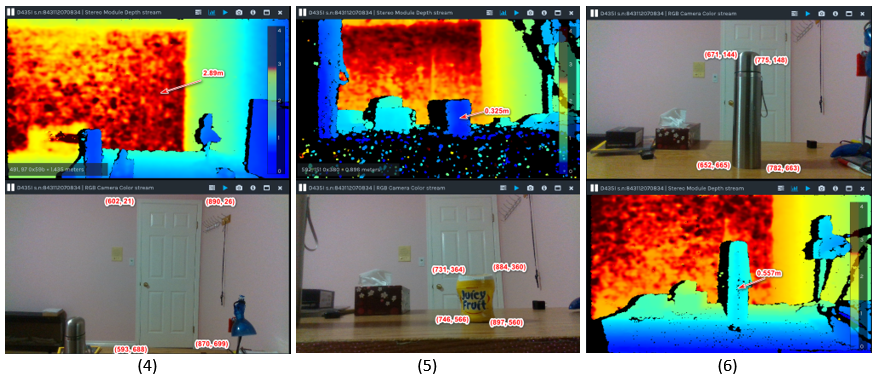
\includegraphics[width=0.9\linewidth]{figures/7} 

}

\caption{Definition of field of view}\label{fig:figure7}
\end{figure}



The comparison of calculation and measurement are as follow table \ref{tab:mytable2} and table \ref{tab:mytable3}, where \[L1 = C \cdot l1 \cdot D1\]

\begin{table}

\caption{\label{tab:mytable2}Information from image}
\centering
\begin{tabular}[t]{lrrr}
\toprule
Item Number & 4.00e+00 & 5.00e+00 & 6.00e+00\\
Depth(mm) & 2.89e+03 & 3.25e+02 & 5.57e+02\\
Height(Pixel) & 6.70e+02 & 2.01e+02 & 5.18e+02\\
Average Ch & 1.09e-03 & 1.09e-03 & 1.09e-03\\
Width(Pixel) & 2.25e+02 & 1.52e+02 & 1.17e+02\\
\addlinespace
Average Cw & 1.10e-03 & 1.10e-03 & 1.10e-03\\
\bottomrule
\end{tabular}
\end{table}

\begin{table}

\caption{\label{tab:mytable3}Measurement Result and Error Rate}
\centering
\begin{tabular}[t]{lrrr}
\toprule
Item Number & 4.00 & 5.0 & 6.0\\
Calculated Height(mm) & 2110.00 & 71.2 & 314.5\\
Actual Height(mm) & 2100.00 & 80.0 & 325.0\\
Error Rate(percentage) & 0.48 & 11.0 & 3.2\\
Calculated Width(mm) & 898.00 & 54.3 & 71.7\\
\addlinespace
Actual Width(mm) & 920.00 & 60.0 & 82.0\\
Weight Error Rate(percentage) & 2.40 & 9.5 & 12.6\\
\bottomrule
\end{tabular}
\end{table}

According to the datasheet {[}7{]} of RealSense Camera, there is a mechanical tolerance of +/-5\% for the camera. Therefore, the error measured is within the tolerance. As we could see, the error will be relatively smaller if the shape of the object is rectangle and facing the camera perpendicularly. Physical measurement on object with anomalous shape will introduce more error compare to rectangles. Also, to simplify the calculation, depth value of the center on the object was taken to calculate the constant C and later the actual height or width. However, the depth value at the center of the water bottle is different from the depth value for the edge. This deviation on depth value will introduce more error. Objects not facing the camera perpendicularly will also introduce errors with the misalignment for the width and height.

To increase the accuracy for the measurement, two optimization strategies could be done. First one is using the average depth value of the object for the calculation. The other method is to calculate the width or height with the coordination in 3D which combines both depth and RGB information.

\hypertarget{combination-of-obstacle-detection-and-trajectory-plan}{%
\section{Combination of Obstacle Detection and Trajectory Plan}\label{combination-of-obstacle-detection-and-trajectory-plan}}

In order to integrate the detected obstacle onto the trajectory plan, the detected obstacle top view will be projected on the map canvas after re-size and rotation. Assuming the camera is facing the destination direction when it is at initial point and the overall canvas has a dimension of 200x200 pixel, the top view obstacle will be re-sized to meet the mapping scale and rotated to the camera orientation. A mask based on the top view frames will be shifted to the start point with the bottom center point coincide with the camera's current position, which is the initial position for now. As there is a new obstacle detected, the trajectory plan function will re-calculate the RRT tree. Figure \ref{fig:figure8} shows the obstacle mask generated with the top view frame from section 3.2 and the RRT calculated with obstacle mask projected on map canvas. The scale for the map canvas is 1:31.25, which means that 31.25 pixels on the map represent 1 meter.

\begin{figure}

{\centering 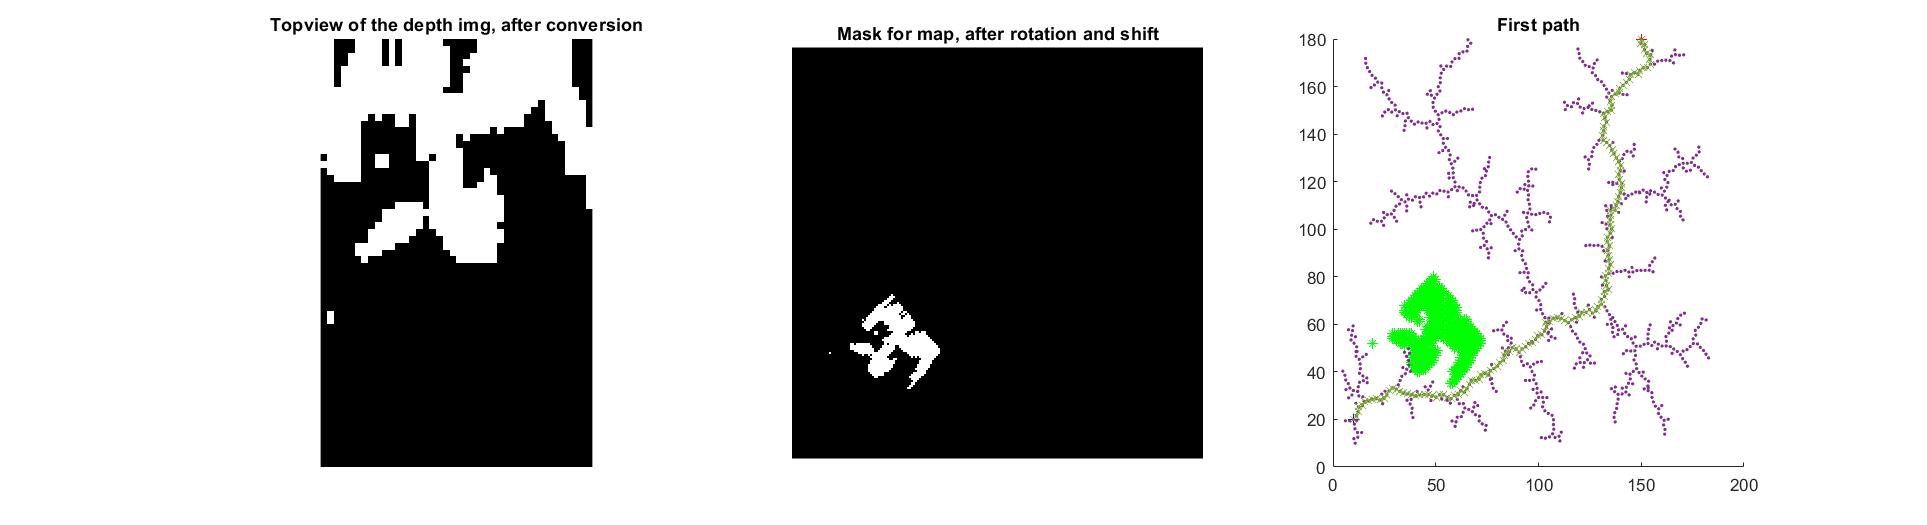
\includegraphics[width=0.9\linewidth]{figures/8} 

}

\caption{Definition of field of view}\label{fig:figure8}
\end{figure}



Later, once the camera starts to move based on the generated path, the object detection and projection will continue. After the initial position, the direction of the camera will be defined by the vector subtraction from current coordinate by previous coordinate. And the mask will be re-size based on the scale, then rotated to the current direction and shifted to the current position. If more obstacles are found since last project, the RRT tree will be recalculated.
In order to increase the safety and avoid the drone being trapped in the anomaly shaped obstacle, a minimum volume ellipsoid has been generated to cover all of the obstacle points as shown in figure \ref{fig:figure9}. The algorithm to find the ellipsoid is discussed in the textbook ``Convex Optimization'' {[}9{]} and the function usage in MATLAB is described in {[}10{]}.

\begin{figure}

{\centering 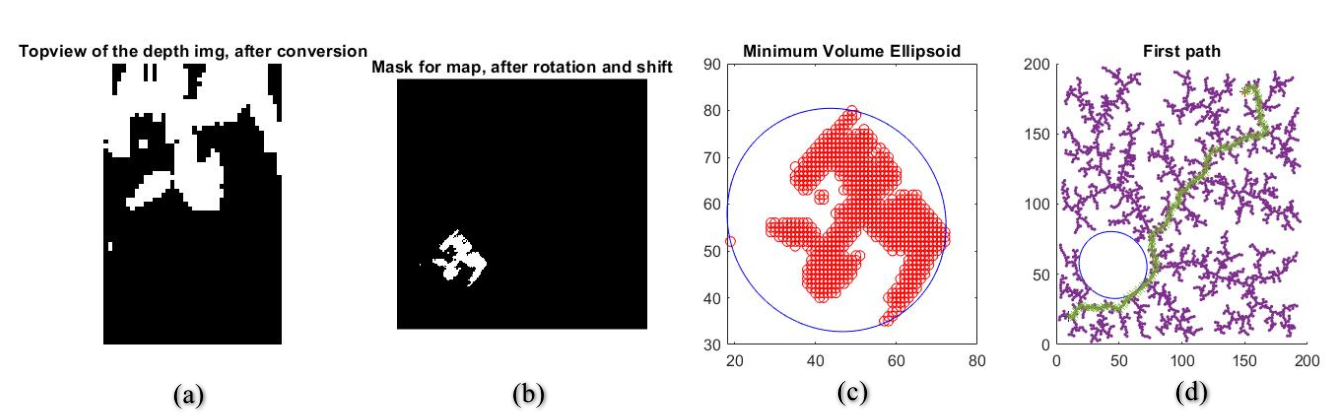
\includegraphics[width=0.9\linewidth]{figures/9} 

}

\caption{Detected obstacle with minimum volume ellipsoid covered}\label{fig:figure9}
\end{figure}



Because of the long RRT calculation time and video processing time, the object will be checked every 5s when the robot's moving speed is 0.1m/s

\hypertarget{update-the-path-as-obstacle-moving}{%
\section{Update the path as obstacle moving}\label{update-the-path-as-obstacle-moving}}

Several scenarios have been demonstrated to prove that the implementation could recalculate the path if the camera detect the object change. Multiple obstacles would show up in the global map as the robot moving along the path. Also, the original obstacles would change the position from time to time. The program would recalculate the RRT tree when changes happen to the environment.

Ideally, the path would only be recalculated when new obstacles are added in the map as shown in figure 2. However, in reality, with the vibration and inaccuracy from the camera, the detected obstacle would change all the time. If the function is set to recalculate the RRT whenever detecting the change in obstacle, it would keep recalculating. Therefore, in the implementation, an update rate has been defined to set the time between the updates of the camera streaming.

The following are two demos on the path updated when new objects detected in figure \ref{fig:figure10} and path updated when object is changed position in figure \ref{fig:figure11}.

\begin{figure}

{\centering 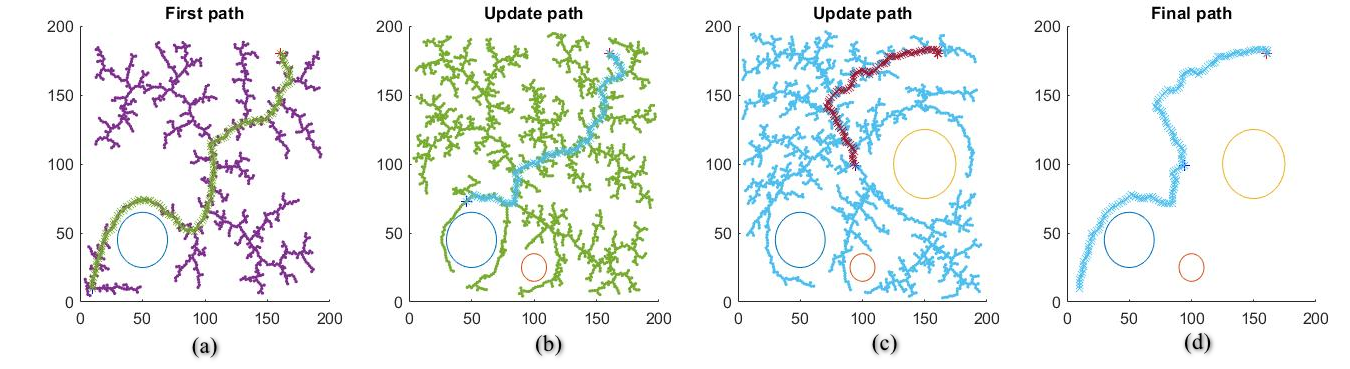
\includegraphics[width=0.9\linewidth]{figures/10} 

}

\caption{Path updated when new objects detected}\label{fig:figure10}
\end{figure}



\begin{figure}

{\centering 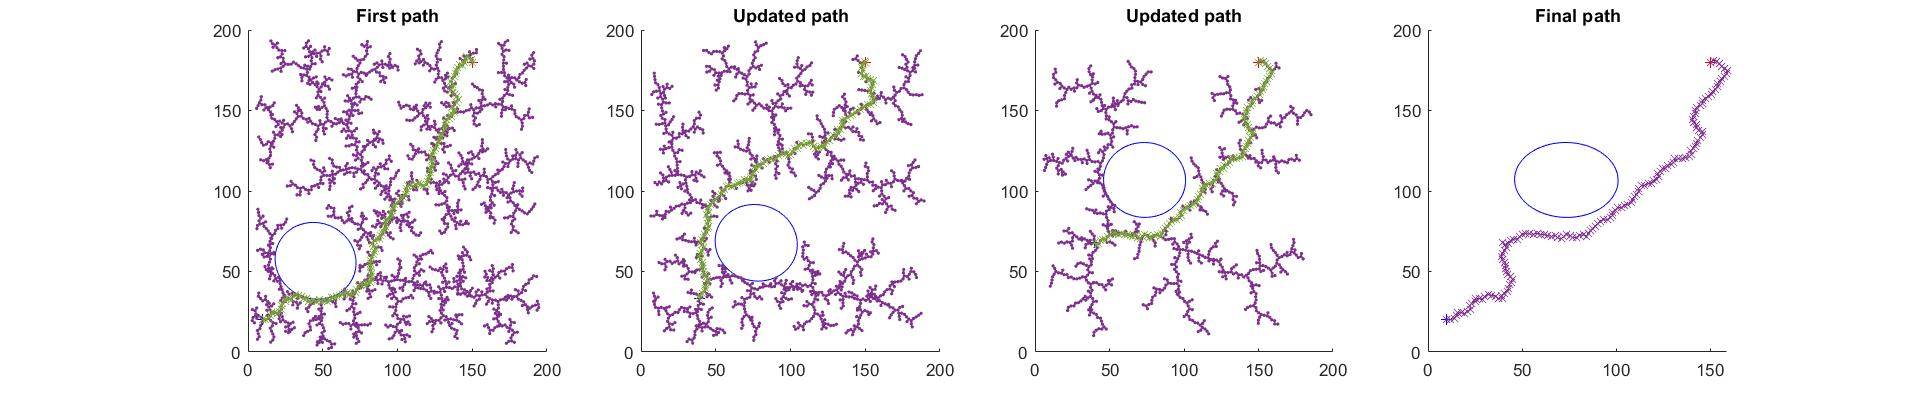
\includegraphics[width=0.9\linewidth]{figures/11} 

}

\caption{Path updated when object moved}\label{fig:figure11}
\end{figure}



The update for the input of obstacles are done by streaming the video separately at different time point. Then feeding these videos are fed into the system which would recalculate the path. This process proves the concept of the capability on updating the obstacles in real time. An actual real time object detection during path planning could be implemented with RealSense SDK in the future.

\hypertarget{discussion}{%
\chapter{Discussion}\label{discussion}}

With the implementation from this project, a trajectory planning methodology that is capable of detecting the obstacle with camera has been implemented. In this section, analysis on the RRT algorithm, error rate and source for the measurement with RealSense camera, limitation for the real-time implementation and future work will be discussed.

The advantage for RRT algorithm is that a collision avoidance path from initial point to the destination would for sure be created, as long as it exists. However, as the algorithm will generate random points to build the tree exhaustively, the computation time will increase dramatically when the obstacles are close to each other on the map. It is important to choose a proper value for the step size between each node on RRT. If the step size is too small, there will be too many nodes to be generated between the two points on the map. This would increase the calculation time. However, if the step size is too large, chances for finding a proper path between obstacles would be decreased, especially for those anomaly shape paths between two obstacles.

The objects captured by the camera were measured. The measurement result defines the scale for transferring the obstacle to the map canvas. In order to increase the accuracy for the measurement, several reference objects have been used for calibration. However, the error rate for the measurement ranges from 0.48\% - 12.6\%. We noticed that when the object to be measured has a flat surface and has a regular shape such as rectangle, the error rate would be lower. And when the object has an irregularly or convex shape such as cylinder, the error rate would be higher. The reason is that the depth information for the flat surface is mostly uniform, but the depth information on the cylindrical surface varying. Current calculation for measurement is based on the depth info at the center point. Therefore, there will be a bias on the depth value. Similarly, the error from varying depth value would be introduced if the surface is not facing the camera perpendicularly. To solve this problem, we could use 3D coordination which combined both RGB and depth information for the measurement.

A limitation for the current implementation is the path planning is not online. Currently, the scripts are importing the recorded video for image processing and object detection. Then the processed result would be imported as obstacle information to the pathway planning algorithm. The video reading process take more than 10s to finish and this set a bottleneck in implementing it in real-time. Also, as the SDK for RealSense camera are mostly implemented with C++, the development environment should be changed to C++ for further implementation.

In the future, there are two main parts to be continued. One is the implement the object detection in real-time with OpenCV packages provided by RealSense. After shifting the C++, combing the object detection with the path planning to allow the algorithm changing the path based on the detected object. The other direction for the future work is the control algorithm for path following. A feedback control algorithm should be implemented to support the done to following the path properly.

\hypertarget{conclusions}{%
\chapter{Conclusions}\label{conclusions}}

The trajectory planning algorithm implemented in this project is capable to detect the obstacle in the camera and generate a pathway to avoid the collision. RRT algorithm has been integrated with the image processing on the video captured by RealSense camera. In the future, control algorithm for path following and object detection in real-time with OpenCV packages should be implemented

  \bibliography{thesis.bib}

\end{document}
